
\chapter{Analysis and planning}

\epigraph{As I see it, criticism is the prime \emph{duty} of the
  scientist and of anyone who wants to advance knowledge. Seeing new
  problems and having new ideas, on the other hand, are \emph{not}
  one's duty: originality is, rather, a gift of the gods.}{Karl Popper
  --- 1982 Preface to ``Quantum theory and the schism in physics''}

\section{Requirement modelling}

In the following section we discuss the requirements that we want to
impose on the resulting framework. Note that functional requirements
are hard to express for an API, but a vague description of the desired
qualities and features is still possible will guide or development
process.

Quite often, we will focus on the final feature that should be
implementable through the framework. Also, note that the framework
already had many features at the beginning of the project, some of
which we will discuss in section \ref{sec:status}. We will try to
avoid describing the requirements related to those ready facilities in
this section, as the only purpose of those is to aid the actual
development of this thesis project. Still, some already satisfied
requirements might be made explicit when some other related
requirement follows, or because of their relevance to the user or just
for the global consistency of the text.

As we suggested in our objective \ref{obj:artquimia}, these
requirements have been elicited with the assistance of the ArtQuimia
Music Production School in order to ensure the suitability of the
software in a productive usage context.

\subsection{Functional requirements}

\subsubsection{Basic audio support}

\begin{requirement}
  \label{req:iter1-begin}
  The library must provide data-structures and basic algorithms for
  manipulating audio signals.
\end{requirement}

\begin{requirement}
  The library must provide means to output and input audio data to and
  from files in various formats, including, at least: Microsoft WAV,
  Apple AU and OGG Vorbis.
\end{requirement}

\begin{requirement}
  \label{req:soundsys}
  \label{req:iter1-end}
  The library must provide means to output and input audio data to and
  from sound-card devices in an asynchronous real-time fashion,
  supporting, at least, the following audio systems:
  ALSA\footnote{Advanced Linux Sound Architecture:
    \url{http://www.alsa-project.org/}}, OSS\footnote{Open Sound
    System: \url{http://www.opensound.com/}}, Jack\footnote{\url{http://jackaudio.org/}}.
\end{requirement}

\subsubsection{Node graph support}

\begin{requirement}
  \label{req:iter2-begin}
  The library must include means for producing the audio as the result of
  executing a dataflow-graph. 
\end{requirement}

\begin{requirement}
  The library user must be able to define his own processing nodes.
\end{requirement}

\begin{requirement}
  \label{req:porttype}
  Each node should have an arbitrary number of named signal and
  control input and output ports. The difference between signal and
  control ports are that the later are sampled at much less frequency.
\end{requirement}

\todo{De hecho, la naturaleza real de las señales de control aún no la tengo
clara al 100\%. Las señales de control son lo que en la versión actual
de GNU/Psychosynth se llaman \emph{parámetros}. Sin embargo, el tema
no es del todo trivial y tras ver como funciona Reaktor y pensar mucho
en como reinventar el MVC del Psychosynth la situación está cada vez
más confusa, pero supongo que la concreción se puede dejar para el
rediseño de esta capa del software en la segunda iteración.}

\begin{requirement}
  Both signal and control ports should be able to process information
  in arbitrary datatypes. Signal ports may have practical limitations
  as for the real-time constraints is concerned.
\end{requirement}

\begin{mynote}[Realtime constraints] \label{note:realtime} All the
  processing done inside the nodes should satisfy soft real-time
  constraints. This is so because in order to produce sound with low
  latency (see requirement \ref{req:latency}) the sound processing
  should be done in blocks (buffers) as small as possible that are
  delivered to the sound-card as soon as possible. If the deadline is
  not met, a disturbing ``click'' sound will be heard because of the
  zeroes assumed by the sound-card during the period that it did not
  have any audio to output. For example, for a 44100 Hz sampling rate
  and a 128 frames block size, it should take less than $$\frac{1
    s}{44100\ frames}\cdot128\frac{frames}{block}=2.90
  \frac{ms}{block}$$ to process and deliver an audio data block.

  In practice, this means that the processing algorithms should take
  an amount of time proportional to the amount of data to process
  ---i.e. they are $O(n)$. This in turn disallows writing and reading
  files and most operations that cause non deterministic hardware
  operations or force context switching (mutexes might be unavoidable
  but should be used scarcely). Also, allocation of memory on the
  heap should be avoided as it has a non-predictable and potentially
  non-linear time consumption. Of course, the framework should provide
  hooks to do those forbidden operations outside the audio processing
  thread, but we consider that a design issue that should be addressed
  later.
\end{mynote}

\begin{requirement}
Each output port must be connectable to arbitrary number of input
ports. Each input port must be connectable to one output port.
\end{requirement}

\begin{requirement}
Ports may be defined statically ---i.e. at compile time--- or
dynamically ---i.e. at runtime.
\end{requirement}

\begin{requirement}
The system must allow the hierarchical composition of nodes, with
special \emph{input} and \emph{output} nodes that are exposed as ports
in the parent level.
\end{requirement}

\begin{requirement}
\label{req:iter2-end}
Nodes can be either monophonic or polyphonic. A polyphonic node
internally has a number of copies of its processing state, called
\emph{voices}, that are dispatched accordingly trough trigger signals.
\end{requirement}

\begin{mynote}[On the scope of polyphony]
We will avoid specifying here details on how polyphony works that are
still quite important as a \emph{usability} concern. For example,
should monophonic ports be connectable to and from polyphonic ports?
Should there be polyphonic and monophonic nodes in the same patch
hierarchy level? How are the voices dispatched and mixed? Because
answering this issue highly affects performance and implementability
tradeoffs, these issues are left open until the design stage of these
components.
\end{mynote}

\subsubsection{Dynamic loading of nodes}

\begin{requirement}
  \label{req:iter3-begin}
  The system must be able to dynamically load modules developed with
  standard interfaces, at least using the LADSPA
  standard\footnote{Linux Audio Developer's Simple Plugin:
    \url{http://www.ladspa.org/}}, but LV2\footnote{LADSPA Version 2:
    \url{http://lv2plug.in}} and VST\footnote{Steinberg's Virtual
    Studio Technology: \url{http://ygrabit.steinberg.de/}} are
  proposed too in this order of priority. Note that in some cases this
  implies the automatic fixing of the semantic impedance among the
  interfaces of Psychosynth nodes and the third-parties'.
\end{requirement}

\begin{requirement}
  The system should be able to dynamically load modules developed
  using the same native interface exposed to library users to define
  their own modules. 
\end{requirement}

\subsubsection{Dynamic patching}

\begin{requirement}
  The system should optionally release the library user from arranging
  the interconnections among nodes by using \emph{dynamic
    patching}. When using \emph{dynamic patching} an output port is
  connected to one input port. The input port is the closest (in the
  sense of euclidean distance, we assume that the modules are laid out
  in the space) input port of the same type not belonging to the same
  node that is free ---i.e. is not connected already to a closer node.
\end{requirement}


When combining dynamic-patching with dynamically loaded modules
using standard interfaces like LADSPA, one might need extra
information to correctly perform the dynamic patching.

\begin{requirement}
  \label{req:iter3-end}
The system should be able to locate and automatically load if present
special description files containing the required information for
some dynamically loaded modules to work correctly. This file should
specify which ports are eligible and to which ports they are
connectable to. 
\end{requirement}

While this may change due to design considerations, we suggest
specifying a set of tags for each port, with the following
connectability rule for port $A$ and $B$: $connectable(A, B)
\Rightarrow tags(A) \cap tags(B) \neq \emptyset$. 

\subsubsection{View independence}

The following requirements are here to suggest an observable interface
for the synthesis model satisfying a model-view-controller
architecture. This is one of the key concepts in achieving a
network-based shared environment that is transparent to a wide range
of graphical interface experiments or external MIDI controls.

\begin{requirement}
  \label{req:views}
  The system must enable the development of graphical interfaces
  ---or any other instance of the more abstract concept of
  \emph{view}--- that can coexist with each-other.
\end{requirement}

\subsubsection{Synchronisation and sequencing}

\begin{requirement}
  \label{req:iter4-begin}
  The system should include a notion of \emph{tempo} such that external
  imprecise events can be quantised and synchronised to.
\end{requirement}

\begin{requirement}
  Parameters of various node kinds, specially time related ones,
  should be controllable as a factor of the current tempo.
\end{requirement}

I.e. the frequency of an LFO should be fixable such that the wave
length is a factor of the tempo, and the phase should be
synchronisable to beat.

\begin{requirement}
  The system should be able to synchronise to the MIDI clock.
\end{requirement}

\subsubsection{Collaborative support}

\begin{requirement}
  The system must be able to receive, process and use as control
  source MIDI events coming from other software or external hardware
  devices.
\end{requirement}

\begin{requirement}
  The system must be able to receive, process and use as control
  source OSC events coming from other software, computers or external
  hardware devices.
\end{requirement}

\begin{requirement}
  \label{req:iter4-end}
\label{req:sharedenv}
  The system must be able to use a specially crafted OSC based
  protocol to enable the collaborative manipulation of the same node
  graph among different computers connected through the network.
\end{requirement}

\begin{mynote}[Relaxing the ``shared-environment'' requirement]
  Requirement \ref{req:sharedenv} is currently implemented by
  broadcasting all events among all the participants in a shared
  session. In presence of audio input nodes, dynamically loaded
  modules and other sources of non-determinism ---this is, sound that
  might not depend only on the sequencing of certain events--- this
  gets harder to implement. We do have some solutions in mind, like
  placeholder nodes that stream the local non-deterministic signals
  through the network too, but it might be too hard to implement in
  the context of this master thesis project and only a
  proof-of-concept implementation will be required.
\end{mynote}


\subsubsection{Persistence}

\begin{requirement}
\label{req:persistence}
The system must be be able to store and load the graph layout and
control values the node graphs. Sub-graphs in the graph hierarchy
should be storable and loadable individually.
\end{requirement}

\subsubsection{Optional functionality}

Requirements in this section are not such, but instead they are bare
ideas that would be nice to have but are considered too time
consuming, hard or not urgent enough to be considered a measure of the
project success.

\begin{requirement}
The highest level part of the API should have a Python ---or any other
dynamic language of choice--- binding for the rapid prototyping of
audio applications and user interfaces on top of it.
\end{requirement}

\subsection{Non-functional requirements}

\subsubsection{Free Software}

\begin{requirement}\label{req:free}
Unless constrained by very specific hardware, the system should not
add any non-Free Software dependency --- i.e, it must be able to
compile and run without executing any privative software bit. 
\end{requirement}

\subsubsection{Professional quality sound}

\begin{requirement}
\label{req:iter1-begin2}
The software must be able to work at different sampling rates up to
96000 Hz.
\end{requirement}

\begin{requirement}
\label{req:iter1-end2}
The software should be able to use arbitrary precision samples. Up to
64 bit floating point samples are required.
\end{requirement}

\subsubsection{Performance}

\begin{requirement}[Latency]
  The software should be able to work with a block size as low as
  possible down to 64 frames, as long as the underlying hardware
  permits it.
\end{requirement}

\todo{En realidad este requisito es un poco ambigüo, pero no se muy bien
  cómo especificar la posibilidad e usar tamaños de buffer bajos, ya
  que las condiciones en las que es medible esto dependen de la
  potencia del procesador y, en un sinte modular que permite redes
  arbitrariamente complejas, del tamaño del sinte. ¿Alguna sugerencia?}

\section{Open, community oriented development}

The developers of this software are strong proponents of Free Software
development. This is specially relevant in an academic and public
environment like ours. Therefore, the software not only is distributed
under a Free Software license, it also follows an open community
development model, where everyone can read, use and modify the
source code as it is developed and there are means for online
communication promoting development among volunteering distributed
peers.

Previous versions of the software are available on the Internet for
download and it has an official web page:
\url{http://www.psychosynth.com}

\subsection{Software License}

The software is licensed under the GPL license version 3, offering
strong copyleft requirements --- i.e. derived works and software
linking against the library must be distributed under the same
terms. The full description of the license is included in the appendix
\ref{sec:license}.

While the GPL3 is often misunderstood as inadequate for a library,
that is not true in the context of libraries that provide unique
features, as it motivates the release of third-party software that is
attracted by these as Free Software too \cite{gnu99why}. This is not
only personal belief, it is also the official guideline in the GNU
project.

\subsection{The GNU project}

Since October 2008, Psychosynth is part of the GNU project. GNU was
started in 1984 by Richard Stallman with the long term goal of
providing a fully free ---as in speech--- operating
system \cite{stallman2002free}. Under the umbrella of GNU, Psychosynth
gets access to a broader community, technical support and it is a
recognition of its attachment to the Free Software ideals.

\subsection{Software forge and source code repository}

A \emph{software forge} is an online service targeted at aiding the
development of Free Software. It offers a series of tools to aid the
community participation and distributed development, such as \emph{bug
trackers}, \emph{support trackers} and \emph{mailing lists}. One of
the most important features is the \emph{revision control system} that
serves as source code repository.

GNU Psychosynth is hosted in the Savannah software forge, and its
project page can be accessed here:

\url{http://savannah.gnu.org/projects/psychosynth}

The project is using GNU Bazaar as distributed revision control
system. One can fetch a copy of the latest version of main development
branch by executing the command\:

\verb!bzr branch http://bzr.sv.gnu.org/psychosynth/trunk!

\subsection{Communication mechanisms}

Fluent distributed communication is essential for the advancement of a
free project. For this purpose we offer the following tools.

\subsubsection{A blog}

The blog serves as an informal and easy way of getting the latest news
on the development. It is most of the time technically oriented and
can serve as source of motivation for external people to contribute to the
project and as a summary of the current status of the project. It can
be accessed through: 

\url{http://planet.gnu.org/psychosynth/}

\subsubsection{Mailing lists}

Mailing lists are multi-directional broadcast based communication
means and the main spot for discussion of development (from the
developer point of view) and getting news or asking for help (from the
spare user point of view).

GNU Psychosynth has two mailing lists.

\begin{itemize}
\item Users mailing list: \\
\url{http://lists.gnu.org/mailman/listinfo/psychosynth-user}

\item Developers mailing list:\\
\url{http://lists.gnu.org/mailman/listinfo/psychosynth-devel}
\end{itemize}

Because being registered in many mailing lists can cause management
issues to some users, the Gmane
project\footnote{\url{http://www.gmane.org/}} offers a newsgroup
gateway that can be used by Free Software projects to allow
participation in their mailing lists with Usenet capable
software. Psychosynth mailing lists are registered there and can thus
be accessed through:

\begin{itemize}
\item \verb|gmane.comp.gnu.psychosynth.user| for the users
  mailing list.
\item \verb|gmane.comp.gnu.psychosynth.devel| for the developers
  mailing list.
\end{itemize}

\section{Development environment}

The development environment is very important for the project
success. This section should clarify our choices and explain the
rationale behind such decisions.

\subsection{Programming language}

Psychosynth is developed using C++. This decision is based on the
following facts:

\begin{itemize}
\item It is a stack based language with fine grained control over
  memory management. As we introduced in note \ref{note:realtime},
  this is crucial during the development of live audio processing
  software.

\item It is a mature language with widespread tool support and a very
  good Free Software compiler: GCC.

\item Apart from its low-level mechanisms it has powerful means for
  abstraction, most of which are designed to pay zero cost.

\item It is multi-paradigm, and as such it can easily adapt to the
  natural way of expressing the concepts of a heterogeneous system as
  this, where we want to go to from low level DSP programming to high
  level interface design.

\item It is compatible with C, which gives us direct access to the
  widest range of libraries available. Most audio-processing libraries
  are written in C and thus we can save a lot of time in
  implementing mathematically complex algorithms. 
\end{itemize}

Of course, it also has its flaws, like unnecessary complexity and
unsafety in some corners, most of which are justified by its backward
compatibility to C and evolutionary design. Some of this flaws are
nonetheless going to be solved in the next standardisation of the
language, to be released in 2011 \cite{herb10iso}.

\todo{Aquí estoy citando un blog --- ¿Es esto correcto o mejor lo pongo como
nota al pie? }

Compilers are starting to support it and we are very interested in
exploring the benefits and new programming patterns and design
benefits that it can provide. Because Psychosynth is an ongoing and
forefront project we do not fear portability --- and after all, GCC is
very portable! --- and as such we are going to use the facilities in
C++0x as soon as they are supported by the latest version of GCC
included in the Debian Sid.

\subsection{Operating System}

The project is mainly targeted at GNU/Linux, which is the most
widespread free operating system, therefore, compliance with it is the
highest priority. That is also the operating system of choice of the
authors of this project so it feels like a natural environment and
there is no extra effort needed.

Still, we will try to comply with POSIX such that porting to other
Unix operating systems is easy. Sadly, there is no universal high
performance and fully featured cross-platform audio output engine and
thus that is an important portability boundary. In the future, maybe
with some financial aid, we might be able to port the software to OSX,
which is near to be the most used operating among
musicians \cite{magnusson07acoustic}\footnote{The cited survey dates
  back to 2006. Given the recent rise in popularity of Apple products,
  we speculate that OSX might be even more popular that Windows among
  musicians nowadays.}.

\subsection{Third party libraries}

In this section we give an overview of the external libraries used in
the software. Note that they have to be chosen in compliance with
requirement \ref{req:free}.

\subsubsection{Boost}

Boost\footnote{\url{http://www.boost.org}} is a set of libraries for
C++ that are peer-reviewed and specially crafted to integrate well
with the paradigms and abstraction techniques of the standard
library. Many of its modules are, actually, going to be part of the
standard library in the future C++0x standard. 

We use few of the Boost facilities, some of them including
\texttt{boost::filesystem}, \texttt{boost::thread}\footnote{We plan to
replace this with the new threading facilities in the standard as soon
as they are implemented in GCC.},
\texttt{boost::mpl}, \texttt{boost::test}\footnote{A wonderful unit
  testing framework.} among others.

It is extremely portable and licensed under the permissive Boost
Software License.

\subsubsection{Libxml2}

We use Libxml2\footnote{\url{http://xmlsoft.org/}} for parsing the XML
configuration files. It is very portable and licensed under the
permissive MIT License.

\subsubsection{LibSndFile}

We use LibSndFile\footnote{\url{http://www.mega-nerd.com/libsndfile/}} for
loading different uncompressed sound formats. Note that from version
1.0.18 it also supports OGG and FLAC formats, and thus we plan to use
this instead of LibVorbis in the future. It is very portable and is
licensed under the LGPL 2 and 3.

\subsubsection{LibVorbis}

We use LibVorbis\footnote{\url{http://xiph.org/vorbis/}} for reading
OGG files. It is released under the BSD license and is very portable.

\subsubsection{SoundTouch}

We use SoundTouch\footnote{\url{http://www.surina.net/soundtouch/}}
for time-stretching, this is, changing the pitch and tempo of a song
independently. It is licensed as LGPL and works on mayor operating
systems.

Some people claim to obtain better results in performance and sound
quality with the Rubber Band
library\footnote{\url{http://www.breakfastquay.com/rubberband/}}
\footnote{The DJ software Mixxx, where sound stretching quality is
  very relevant, is moving towards RubberBand and their developers
  support the above claims:
  \url{http://www.mail-archive.com/mixxx-devel@lists.sourceforge.net/msg03103.html}

  Also, Ardour later moved tater moved to this library:
  \url{http://www.ardour.org/node/1455}} and we will probably replace
SoundTouch by this one in the future.

\subsubsection{ALSA, OSS and Jack}

In accordance to requirement \ref{req:soundsys} we use ALSA, OSS and
Jack respectively. Licenses are LGPL2+ for all of them. ALSA is Linux
only, Jack works on GNU/Linux and OSX and OSS works on Linux and some
other POSIX operating systems.

\subsubsection{LibLO}

LibLO\footnote{\url{http://liblo.sourceforge.net/}} is used for OSC
support. It is licensed as LGPL2+ and is POSIX compliant.

\subsubsection{The user interface libraries}

The user interface included at the beginning of the project is based
on Ogre3D\footnote{\url{http://www.ogre3d.org/}}, using
OIS\footnote{\url{http://www.ogre3d.org/}} (Open Input System) for
keyboard and mouse input and
CEGUI\footnote{\url{http://www.cegui.org.uk/}} as widget toolkit.

During the development of the previous Psychosynth versions CEGUI has
proven to be extremely painful with an overengineered API and bugfull
implementation. Also, the 3D interface, while being fancy it is
confusing for some users and did not offer anything new to the
experienced musician, as some blog reviews showed. It contains some
interesting concepts --- zoomability being the most important --- but
it is too distracting after-all. Thus, while we are going to keep this
interface during the development of this project, we want to later
rebuild the GUI using Qt, which is multi-touch enabled and could open
us the door to the yet-to-come wide range of Meego based tablets.

\subsubsection{Build system}

We use GNU Autotools\footnote{We use mainly Autoconf
  (\url{http://www.gnu.org/software/autoconf/}), Automake
  (\url{http://www.gnu.org/software/automake/}), and Libtool
  (\url{http://www.gnu.org/software/libtool/}).} as the build system
for the project. It is extremely portable and the de-facto standard
among Free Software, even though some interesting alternatives are
emerging. Nonetheless, Autotools are suggested in the GNU Coding
Standards\cite{stallman10coding} that we shall follow during our
development due to our affiliation to GNU.

\subsubsection{Documentation system}

Because we are developing a framework, it is specially important that
the public interfaces are properly documented. We are going to use
Doxygen\footnote{\url{www.doxygen.org}} to embed the API documentation
in code comments. A reference manual generated by Doxygen should be
attached to this document.

\section{Architecture and current status}

The Psychosynth project was started in 2007 and since there has been
some relevant developments. The screenshot in figure
\ref{fig:screenie} gives a broad perspective of the current features
of the project. For a more detailed description from the user point of
view, please refer to the user manual that can be checked online on
the project
webpage\footnote{\url{http://psychosynth.com/index.php/Documentation}},
where there are also demonstration videos and other multimedia
material. The article \cite{bolivar08psychosynth} can serve as an
introduction to the project too.

\begin{figure}[h!]
  \centering
  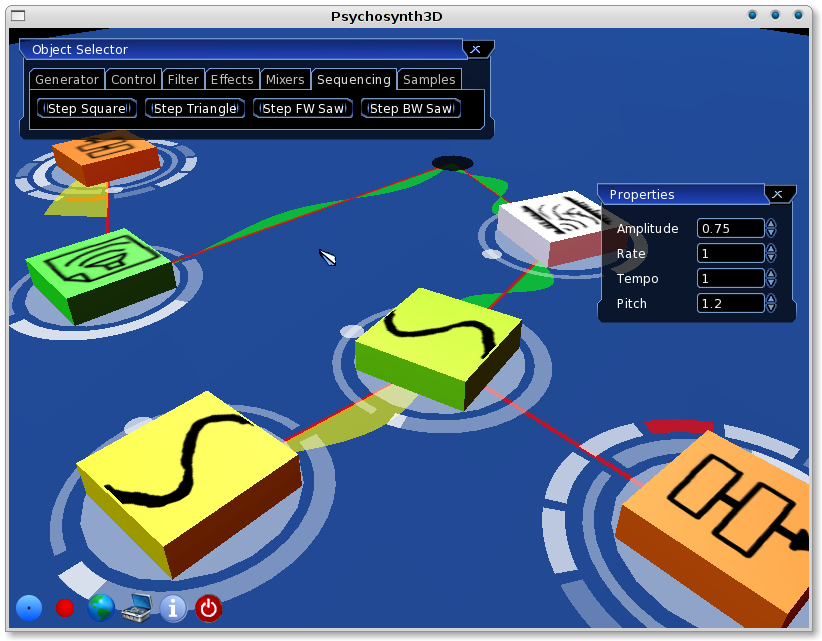
\includegraphics[width=.7\textwidth]{pic/screenie.png}
  \caption[A screenshot of GNU Psychosynth 0.1.4]{A screenshot of GNU
    Psychosynth 0.1.4. On the bottom we can see some buttons for
    poping up different menu windows, such as for settings, recording
    the sound into a file or connecting several instances over the
    network. The window on the top of the screen is used to add
    elements to the processing graph. The smaller \emph{properties}
    windows contains a listing of all the actual parameters of a node
    and allows us to give numeric values to them. All around the
    screen, sinusoids, step sequencers, file samplers and echo filters
    are interconnected as represented by the 3D blocks.}
  \label{fig:screenie}
\end{figure}

\subsection{A critique on the term framework}

The term \emph{framework} is used many times in this and other
projects and is becoming a techie buzzword. In many contexts it is
abused as a synonym for the term \emph{library}. Instead, we believe
that a framework is something different, following the definition
given in the famous design patterns book by the gang of
four \cite{gamma95design}.

We use the term \emph{library} when the root of the call graph is on
the client side and she invokes the library function sparely to obtain
some concrete functionality. Instead, a \emph{framework} stands in the
root of the call graph and the client code is called through extension
hooks in the framework, following the ``Hollywood principle'' ---
``Don't call us, we'll call you.''.

Because the Psychosynth system is layered, one can just use the bottom
layers as a library, or rely on the upper layers that properly use
inversion of control like a framework.

\subsection{The layered architecture}

At the current stage, GNU Psychosynth implements a layered
architecture \cite{garlan94software}. This intends to promote a more
decoupled design, as calls between modules are only allowed from top
down.

Also, the library has many features, many of which some users may
not need. This layered approach could allow a potential user to avoid
any special overhead when he is only using some bottom layers. Still,
note that the library is now compiled will all layers bundled in the
same shared-object file, so this is not a fact now. Because the heavy
redesign ongoing during this project, we shall postpone that until the
late development stages when the layer interactions are clear and
stable.

Figure \ref{fig:layers} represents the current layered
architecture. Lets make a bit more in-depth discussion of each layer.

\begin{figure}[h!]\centering
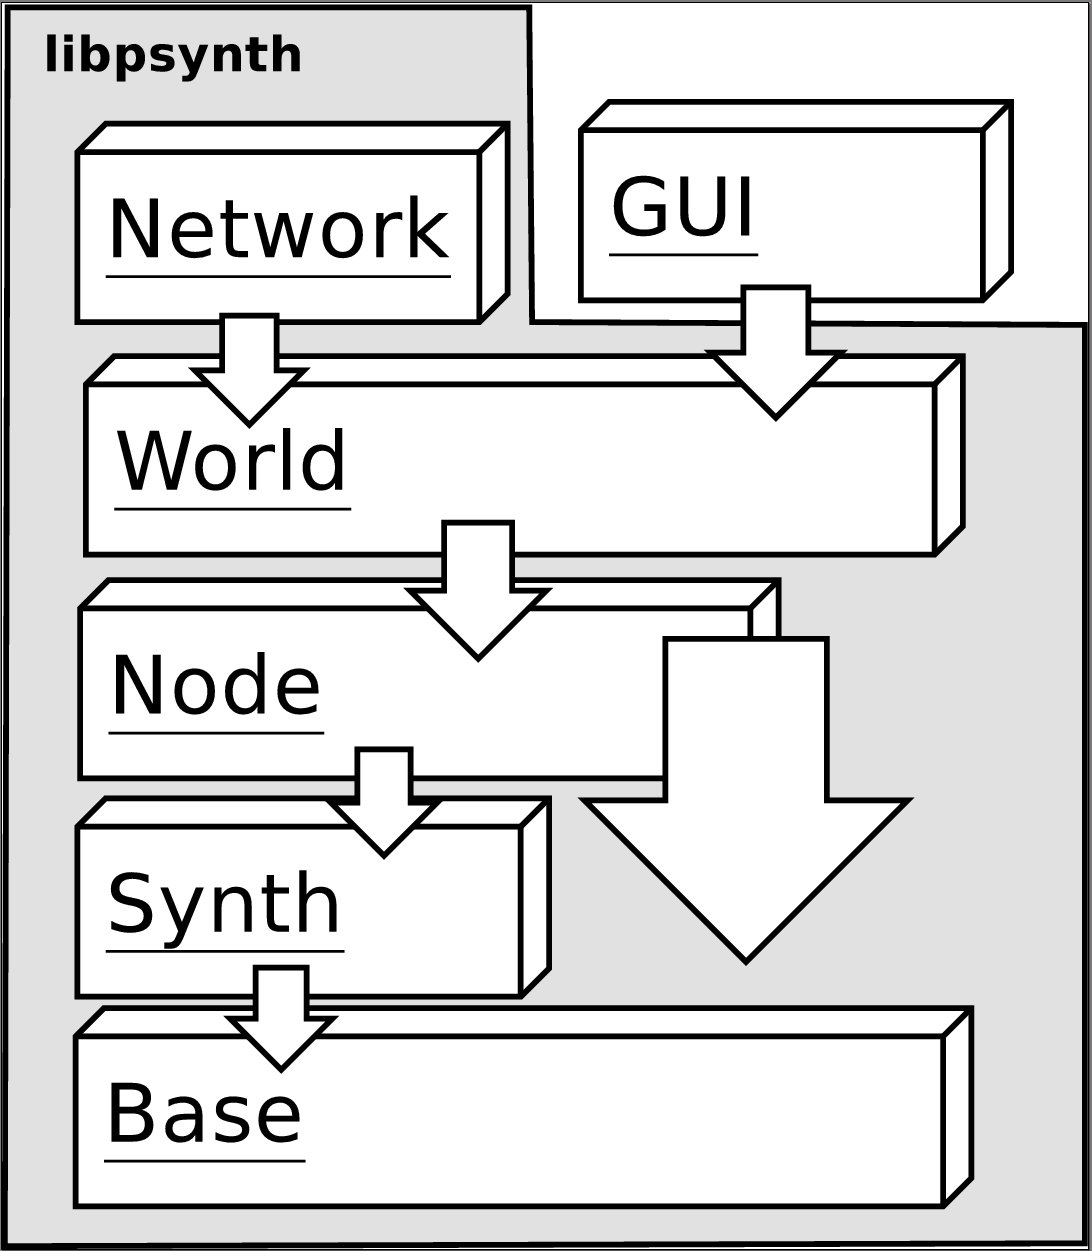
\includegraphics[width=.4\textwidth]{pic/layers.png}
\caption{The Psychosynth layered architecture.}
\label{fig:layers}
\end{figure}

\subsubsection{The \texttt{base} layer}

The base layer includes basic facilities that may be reusable in any
other part of the application. Some of the most relevant examples:

\begin{description}
\item[Configuration persistence] Classes for representing program
  settings in a hierarchical manner. This configuration system can use
  interchangeable backends and has an observable
  interface.\footnote{We use quite often the term \emph{observable
      interface} which is rare in the literature. By this, we mean
    that it provides signals, listeners or other event mechanisms,
    instances of the \emph{observer} design
    pattern\cite{gamma95design}.}

  In fact, we do not recommend using this module in the core of the
  intermediate layers of the library because it can cause unexpected
  coupling, but this is not too clear and we keep it here for
  historical reasons.

\item[Implementation of design patterns] While the term \emph{design
    pattern} means reusable design structure, not reusable code,
  language abstractions can make them implementable as code in some
  cases. Andrei Alexandrescu proves this point for C++ in
  \cite{alexandrescu01modern}. Thus, we provide implementations, quite
  often similar to Alexandrescu's, to various recurring design
  patterns such as \emph{factory} or \emph{singleton}. Some
  implementations are not inspired in Alexandrescu's, like the generic
  \emph{composite}.

\item[Command line argument parsing] While we have considered moving
  to Boost's Program Options library, our own implementation have
  different trade-offs and is rather extensible.

\item[Logging system] A hierarchical and multi backend logging system
  for registering messages from other modules. It should be used
  instead of direct output to \texttt{std::cout/cerr} in all the code.

\item[File management tools] That ease the task of finding resources
  in the hard-drive and can cache results.
\end{description}

Some other minor classes and tools are excluded from this list. During
the development of the project we will drop in this layer classes that
feel interesting at any abstraction level.

\subsubsection{The \texttt{synth} layer}

This layer contains classes for the \emph{static} construction of
synthesisers and sound processing. The audio input and output
facilities are considered to be in this layer, and as well audio
processing data structures ---like ring buffers, multi channel
buffersm, etc.---, basic implementations of filters, oscillators and
audio scalers.

By static, we mean that this code does not provide any dynamic routing
facilities, instead, the programmer is in charge to assign buffers and
call the processing elements manually.

Requisites \ref{req:iter1-begin} to \ref{req:iter1-end} should be
implemented here. Non functional requisites \ref{req:iter1-begin2} to
\ref{req:iter1-end2} are specially relevant in this layer too.

\subsubsection{The \texttt{node} layer}

This layer provides the facilities for the \emph{dynamic} construction
of synthesisers. It includes the mechanisms for describing and
executing the modular synthesis graph with the signal flow and so
on. Figure \ref{fig:node} represents the main concepts behind the
current design. Ports are considered as ``signal ports'' using the
terminology in requirement \ref{req:porttype} --- ``control ports''
are similar to ``parameters'', but parameters are not a precise model
of ``control ports'' as they can not be routed and are intended for
communication between the client user interface code and the audio
thread state.

The communication system used to propagate values between the audio
processing thread and the client thread is represented in figure
\ref{fig:thread}. Values are copied to and from an intermediate channel
between the audio processing blocks. 

\begin{figure}[h]
\centering
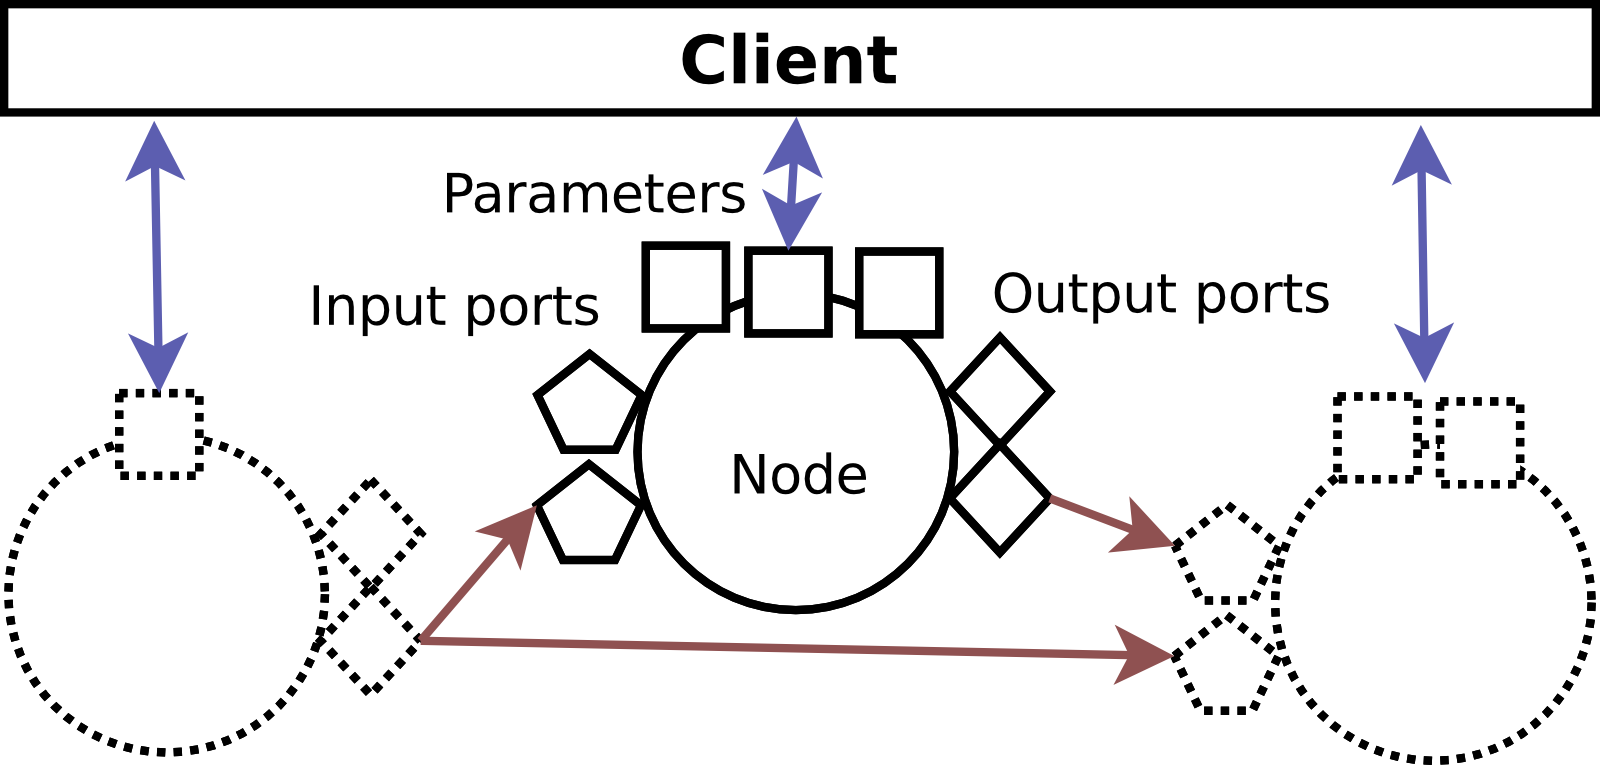
\includegraphics[width=.6\textwidth]{pic/node.png}
\caption[Representation of the node graph as in Psychosynth
0.1.7]{Representation of the node graph as in Psychosynth 0.1.7. Input
ports are represented as pentagons, output ports as rombus and
parameters as squares.}
\label{fig:node}
\end{figure}

\begin{figure}[h]
\centering
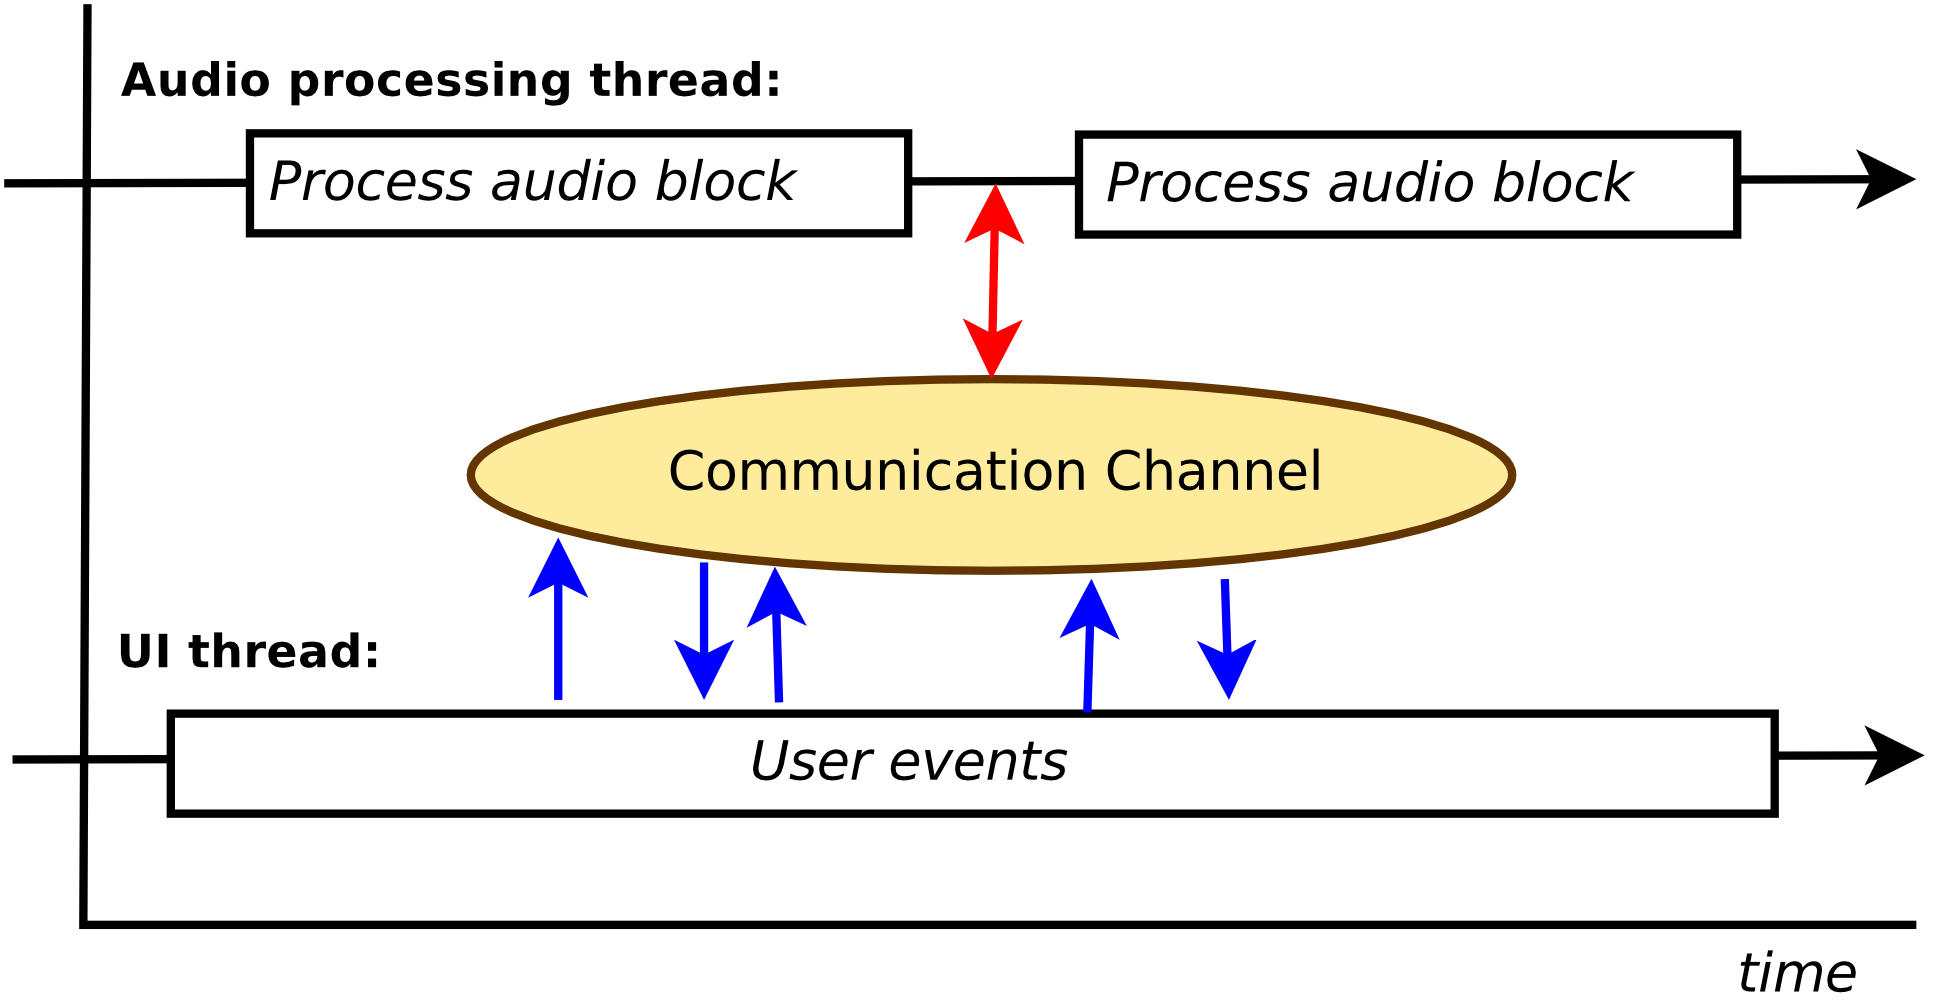
\includegraphics[width=.7\textwidth]{pic/thread.png}
\caption{Communication between the audio and user interface thread as
  in Psychosynth 0.1.7}
\label{fig:thread}
\end{figure}

Requisites \ref{req:iter2-begin} to \ref{req:iter2-end} should be
implemented in this layer. A heavy redesign of its API and many of its
internal implementation is to be expected for that to be accomplished.

\subsubsection{The \texttt{world} layer and the Model View Controller
  architecture}

This layer simplifies the interface exposed to the previous layer and
makes it \emph{observable}. This is fundamental for the Model View
Controller that the system implements.  Figure \ref{fig:mvc}
represents this architectural style. On the following, we can refer to
this observable interface abstracting the synthesis engine as
\emph{the model}.

\begin{figure}[h!] \centering
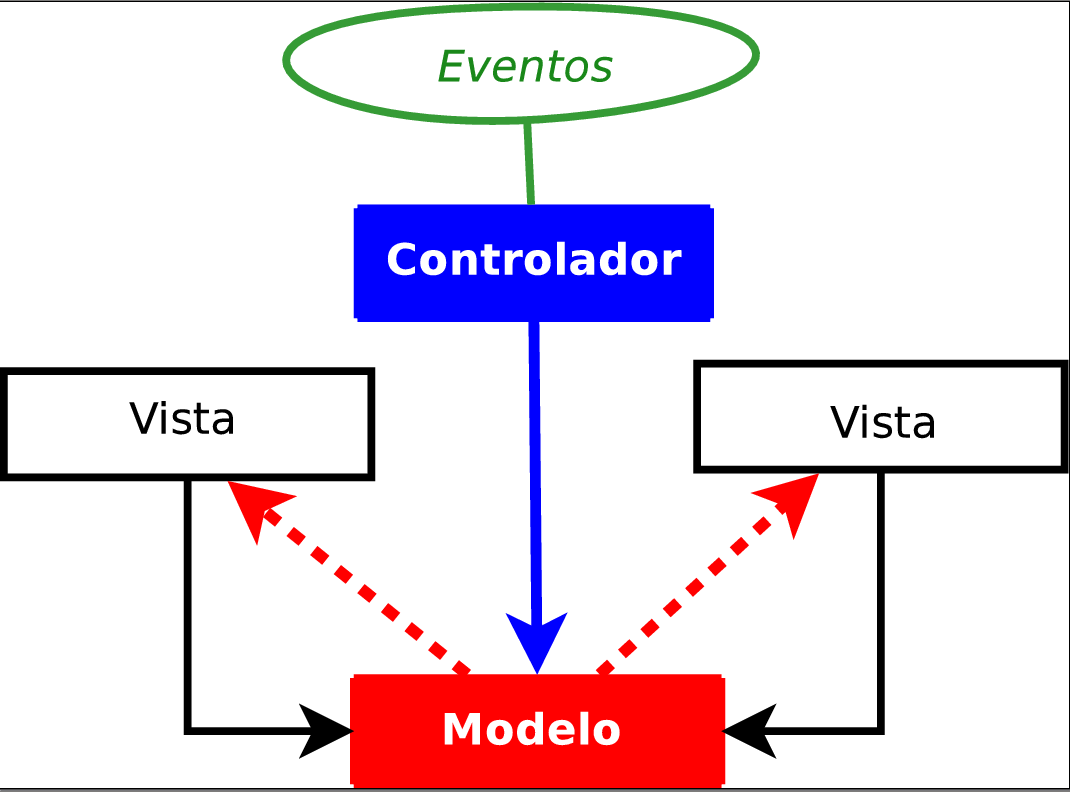
\includegraphics[width=.5\textwidth]{pic/mvc.png}

\todo{Mejorar y traducir esta figura.}

\caption[The MVC architectural style]{The Model View Controller
  arquitectural style. Dashed arrows represent indirect invocation
  ---i.e. via the \emph{observer} design pattern--- and normal lines
  represent normal method calls and data access.}
\label{fig:mvc}
\end{figure}

Several views can coexist independently ---for example, a GUI user
interface and a web client---, that get updated whenever a value has
changed in the model. They register themselves on the model at the
beginning and then become passive entities that get called by the
model. The model changes when controllers invokes methods on it,
several controllers can coexists too. Usually, models and views come
in pairs. For example, a GUI view has an associated controller that
triggers the manipulation of the model in the eventuality of certain
user actions like clicking a button; in this case the representation
(the buttons) and the action (clicking it) are strongly related, but
this is not necessarily true for other situations.

This layer also abstracts the graph interconnection mechanism using
the \emph{strategy} design pattern. Concretely, dynamic patching is
implemented here and the interface exposed in this layer hides the
manual node interconnection mechanisms but provides observability for
topological changes.

This layer should implement requisite \ref{req:views}. 

\subsubsection{The application framework layer and the view and
  controller layers}

There is a thin layer, instance of the \emph{facade} pattern, called
\texttt{app}, that was hidden for simiplicity in figure
\ref{fig:layers} representing the layered architecture. It sits on top
of the \texttt{world} layer and is in charge of initialising the
\emph{world} and defines a configuration tree, using the facilities in
the \texttt{base} layer, and setups the machinery using the
observability of the configuration system to keep coherence between
the user preferences and the status of the synthesis model --- for
example, if the ``\texttt{psynth.output}'' setting is changed, it
automatically creates the appropriate output object instance, sets its
values and substitutes the output node in the synthesis graph. This
layer also sets up the command line argument parsing and installs some
common audio setting arguments in the parser. This layer is where
Psychosynth becomes a framework at its most pure level, as it offers a
\texttt{psynth\_app} class whose \texttt{run} method
should be the only call in the program \texttt{main}, and in turn
delegates the heavy work to user code that is hooked as method
overrides of that same class.

Orthogonal to this layer and sitting also on top of the \texttt{world}
layer the networking layer offers a set of views and
controllers\footnote{A primitive implementation of such at this stage
  of the development.}  that can be used to create the shared
environment described in requirement \ref{req:sharedenv} and thus
allowing collaborative performances. This is an example of the value
of the MVC architecture: because views and controllers are orthogonal,
the user interface does not need to know about the presence of this to
function properly; one could develop a new experimental and cool UI
and it would automagically be able to work with third party clients
over the network, even potentially using a different user interface.

On top of all this there is in the current version of Psychosynth the
code of the 3D user interface and small and simple command line tools
intended to be used as GUI-less network capable clients and
servers. But all this code is not part of the framework, as it wants
to be user interface agnostic, so we will not further describe that
code.

\section{Project planning and methodology}

\subsection{Rationale --- A critique on software engineering}

\todo{Lo se, soy un criticón enfermizo. He acabado convirtiendo esta
  sección en una crítica (indirecta y relativamente elegante, espero)
  a la concepción de la ingeniería del software que se da en la
  facultad y que se hace a menudo de los PFC. Si pensáis que esta
  crítica es demasiado larga o inapropiada puedo matizarla o
  eliminarla :D No obstante, en su defensa la considero apropiada ya
  que la elección de una metodología debe ser racional y como tanto
  debe incluir un análisis crítico de las alternativas.}

Choosing a well known software engineering process is considered one
of the first steps to be taken in a final master thesis project. In
our school we study with most detail the Cascade Process and the
Unified Rational Process.

Those development processes propose a fordist software production
model, targeted at huge development teams and the development of
stable code bases in non innovative well defined fields. Martin Fowler
makes a great point \cite{fowler01design} criticising the often
repeated argument stating that software engineering is like any other
engineering where creative analysis and design is only the first step
and thus coding is analogous to construction. As he says, the
construction is done by the compiler and people involved in
programming are actually doing an intellectual and creative work too
--- in computing, any systematic task can and must be automated. The
$programming=construction$ metaphor is alienating for the programmer,
who is completely excluded from the task of criticising and improving
the software design, and thus this metaphor often leads, in the end,
to bad software.

Moreover, fordist development models take risk control and client
requirements satisfaction as most important factors. Because we are in
an academic environment, there are two more important factors: the
pedagogical value of the project ---this is, that the student involved
takes the risk of exploring the unknown by himself--- and the research
value ---this is, that the student involved takes the risk of
exploring the unknown by humanity.

Of course, this is neither a pure research project, so we can not
substitute a software development project by the scientific
method. But we can choose a more dynamic methodology that includes
\emph{falsification} in one way or the other; \emph{agile}
methodologies\footnote{\url{http://agilemanifesto.org/}} propose many
alternatives that could be valid for a master thesis project.

Still, these methodologies are, we believe, inadequate for this
concrete project. The main reason is that this project is developed by
only one person. Most methodologies, specially agile ones, put
emphasis on the developer communication methods and collective
decision making, so they are often inadequate and too constraining and
time consuming for an unipersonal team.  The Personal Software
Proccess \cite{watts96psp} proposes a methodology that is specially
targeted at personal software developed by engineering
students. Sadly, we are not very familiar with it ---and do not have
enough time to make that happen within the time constraints of the
project--- and it seems too be to specific and time consuming in its
time tracking proposal.

Because we still believe that some rational planning and methodology
is needed, we propose in the following a defined but unconstrained
methodology that is specially tailored for our circumstances,
capturing the most common elements in other software processes.

\subsection{An iterative development model}

Because of the size and complexity of the project, we should not
consider developing it all at once. Moreover, the layered architecture
of the starting code base and the variety of requirements that we want
to satisfy favour an iterative development.

For all this, we want to split the development in iterations. Each
iteration is composed by the following phases:  \emph{design},
\emph{implementation}, \emph{verification} and
\emph{integration}. Each iteration shall be assigned a set of
requirements from the specification in section \ref{sec:requirements}
that are to be satisfied after the successful accomplishment of that
iteration.

\subsubsection{The design phase}

In the design phase we shall define the API that we would like the
current subsystem have. Because we are developing a library and
framework with a public interface, the design phase is specially
relevant shall be done with care.

We do not enforce a particular method for documenting the design as
different paradigms favour different documentation means. For example,
in the first iteration we will develop a library heavily based on
metaprogramming, where UML does not fit very naturally. Still, the
documentation should include rationale explaining why the design
decision lead to the satisfaction of the requirements that we want to
satisfy after this development iteration. Also, it may be found that a
requirement may be impossible to satisfy on the current iteration or
that this requirement is to be better integrated in some other
iteration. The developer is free to reassign that requisite for later
iteration properly documenting this as a post-analysis plan fix.

What we do enforce is that all the API is documented with Doxygen for
the sake of completeness of the reference manual that you should
receive along with this document.

\subsubsection{The implementation phase}

During the implementation phase the code implementing the design
should be written. It is possible and even recommended to modify the
design during this phase as inconsistencies and fundamental problems
are found. Sometimes, this may even start as soon as design, specially
when it is unclear the properties that such API should have and some
``exploratory programming'' is needed. This fact may or many not be
documented at the beginning of the section --- even though an API may
be designed through an inductive empirical process, a deductive
rational description may be more useful for its clear understanding.

\subsubsection{The verification phase}

In the verification phase we perform \emph{unit tests} on the most
important parts of the system. No iteration should be considered
finished unless proper unit tests are written and satisfied for its
core components. For writing such tests the Boost Unit Testing
Framework should be used.

When some elements are considered relevant to performance
requirements, \emph{performance tests} should be included. While we do
not enforce a specific performance testing technique here, the
tests should be reproducible and automatable whenever possible.

\subsubsection{The integration phase}

When a subsystem is added and it is to replace an existing subsystem
in the project, the older code should be removed and the layers on top
modified such that they use the new code. This might even be
considered part of the verification, as older tests working on the
upper layers should be checked to be working still.

Informal integration tests should be done on the final user interface
to make sure that the older properties are preserved. Note that in
most cases, we do not recommend to lose time editing the old user
interface such that the new features in the framework are exposed to
the user. Of course, that the new features are usable is the final
objective, but as it was justified in \ref{sec:userinterface}, a
completely new user interface will be developed as part of a future
project.

\subsubsection{Recursive decomposition of iterations}

In practice, some of the expected requirements to be satisfied may be
found orthogonal or maybe too big to be addressed at one. It is thus
allowed to recursively decompose an iteration in sub-iterations when a
first evaluation during the design phase suggests that.

\subsection{A project plan}

\subsubsection{First iteration: A metaprogramming based sound
  processing foundational library}

This iteration is here to deeply re-design the core data structures
using the latest techniques in C++. This requires special research and
performance requirements deeply rely on the success of this
iteration. 

Requirements \ref{req:iter1-begin} to \ref{req:iter1-end} and
\ref{req:iter1-begin2} to \ref{req:iter1-end2} should be satisfied for
its success.

Etimated time cost: 6 weeks.

\subsubsection{Second iteration: Redesign of the \texttt{node} layer
  for hierarchy and polyphony}

The \texttt{node} layer requires a redesign if we want to satisfy all
our purposes. Polyphony and hierarchy would be specially tricky to
implement directly on top of the current code base. A special
evaluation of how the new design interacts with the MVC architecture
and networking is required. The \texttt{world} layer may be affected
too. All the design changes should be implemented too.

Requirements \ref{req:iter2-begin} to \ref{req:iter2-end} should be
satisfied for its success. Requirement \ref{req:persistence} may be
considered for its implementation in this iteration too.

Estimated time cost: 6 weeks.

\subsubsection{Third iteration: Dynamic loading of nodes}

In this iteration the plugin system is to be developed.

Requirements \ref{req:iter3-begin} to \ref{req:iter3-end} should be
satisfied for its success.

Estimated time cost: 4 weeks.

\subsubsection{Fourth iteration: Adding MIDI and synchronisation}

Synchronisation and MIDI support is one of the most important
features and it is also one of the features we know the least about,
thus, we should put special care on research and design. This will
affect the node and world layers mostly.

Requirements \ref{req:iter4-begin} to \ref{req:iter4-end} should be
satisfied for its success.

Estimated time cost: 8 weeks.

\subsubsection{Post mortem analysis}

After the conclusion of all the previous iterations, we should write a
conclusive report and evaluation of its success. Also, we should
prepare a final presentation for its evaluation.

%%% Local Variables: 
%%% mode: latex
%%% TeX-master: "00-main"
%%% End: 
